%%
%% This is file `./samples/shortsample.tex',
%% generated with the docstrip utility.
%%
%% The original source files were:
%%
%% apa6.dtx  (with options: `shortsample')
%% ----------------------------------------------------------------------
%% 
%% apa6 - A LaTeX class for formatting documents in compliance with the
%% American Psychological Association's Publication Manual, 6th edition
%% 
%% Copyright (C) 2011-2017 by Brian D. Beitzel <brian at beitzel.com>
%% 
%% This work may be distributed and/or modified under the
%% conditions of the LaTeX Project Public License (LPPL), either
%% version 1.3c of this license or (at your option) any later
%% version.  The latest version of this license is in the file:
%% 
%% http://www.latex-project.org/lppl.txt
%% 
%% Users may freely modify these files without permission, as long as the
%% copyright line and this statement are maintained intact.
%% 
%% This work is not endorsed by, affiliated with, or probably even known
%% by, the American Psychological Association.
%% 
%% ----------------------------------------------------------------------
%% 
\documentclass[jou]{apa6}

\usepackage[american]{babel}

\usepackage{csquotes}
\usepackage[style=apa,sortcites=true,sorting=nyt,backend=biber]{biblatex}
\DeclareLanguageMapping{american}{american-apa}
\addbibresource{bibliography.bib}


%%%%%%%%%%%%%%%%%%%%%%%%%%%%%%%%%%%%%%%%
%% Discrete Structures
%% The start of RBS stuff
%%%%%%%%%%%%%%%%%%%%%%%%%%%%%%%%%%%%%%%%

% Working internal and external links in PDF
\usepackage{hyperref}
% Extra math symbols in LaTeX
\usepackage{amsmath}
\usepackage{gensymb}
\usepackage{amssymb}
% Enumerations with (a), (b), etc.
\usepackage{enumerate}

\let\OLDitemize\itemize
\renewcommand\itemize{\OLDitemize\addtolength{\itemsep}{-6pt}}

\usepackage{etoolbox}
\makeatletter
\preto{\@verbatim}{\topsep=3pt \partopsep=3pt }
\makeatother

% These sizes redefine APA for A4 paper size
\oddsidemargin 0.0in
\evensidemargin 0.0in
\textwidth 6.27in
\headheight 1.0in
\topmargin -24pt
\headheight 12pt
\headsep 12pt
\textheight 9.19in



\title{Quiz for Week02}
\author{Discrete Structures, Fall 2020}
\affiliation{RBS}

\leftheader{Discrete Structures (W2): Quiz}

\abstract{%
}

%\keywords{}

\begin{document}
%\maketitle

\twocolumn
{\Large Discrete Structures (W2): Quiz}

\thispagestyle{empty}

\vspace{6pt}
{\bf Question 1.} Let $p \in \mathbb{Z}^{+}$ be a positive integer.
Translate into predicate logic: ``$p$ is a prime number.'' (Prime numbers
have exactly two positive divisors: $1$ and the number itself).\\
{\em Note.} Use ``infix'' notation in your expressions: write 
$a\,\mid\,b$ whenever $a$ divides $b$; write $x < y$, if $x$ is less than $y$.

{\scriptsize \em (Write predicate expression; specify domains for quantifiers.)}

% box for an answer

\vspace{40pt}
{\bf Question 2.} We define $P(n)$ to be true
iff $n$ is a prime. For example, 
$P(2)$, $P(3)$, $P(5)$ etc.\ are true,
but $P(1)$, $P(4)$ etc.\ are all false.\\
Translate into predicate logic: ``There are arbitrarily large primes'', i.e.\ there is no 
such thing as the largest prime.
(Use just the $P(n)$ and inequaly symbols as predicates.)

% box for an answer
\noindent
{\scriptsize \em (Write predicate expression; specify domains for quantifiers.)}



\vspace{40pt}
{\bf Question 3.} You can express the exclusive OR as a {\em disjunction of conjunctions}:
$$a \oplus b \;\equiv\; (a \wedge \neg b) \vee (\neg a \wedge b).$$ 
Indeed, for $a \oplus b$ to be true, you should 
either have $a$ true and $b$ false: $(a \wedge \neg b)$ or 
$a$ false and $b$ true: $(\neg a \wedge b)$. 

Express this truth table as a {\em disjunction of conjunctions} as well \textendash{}
list all cases when it takes value {\tt T}:

\begin{tabular}{ c | c | c | c }
$p$ & $q$ & $r$ & $E(p,q,r)$ \\ \hline
{\tt T} & {\tt T} & {\tt T} & {\tt T} \\ \hline
{\tt T} & {\tt T} & {\tt F} & {\tt F} \\ \hline
{\tt T} & {\tt F} & {\tt T} & {\tt F} \\ \hline
{\tt T} & {\tt F} & {\tt F} & {\tt F} \\ \hline
{\tt F} & {\tt T} & {\tt T} & {\tt F} \\ \hline
{\tt F} & {\tt T} & {\tt F} & {\tt T} \\ \hline
{\tt F} & {\tt F} & {\tt T} & {\tt F} \\ \hline
{\tt F} & {\tt F} & {\tt F} & {\tt T} \\ \hline
\end{tabular}

\noindent
{\scriptsize \em (Write Boolean expression as disjunction of conjunctions)}




\vspace{40pt}
{\bf Question 4.} There are altogether $10$ children: $\{ c_1,\ldots,c_{10} \}$ and 
$10$ hats: $\{ h_1,\ldots,h_{10} \}$. Initially, every child $c_i$ has his own hat $h_i$.
When they were about to leave a party, there was an electricity 
blackout, and they grabbed hats at random (not necessarily their own). 
Predicate $G(i,j)$ is true iff child $c_i$ grabbed hat $h_j$.\\
{\bf (a)} Write the domain set and the range set of the 
predicate function $G$.\\
{\bf (b)} Translate this statement into predicate logic: ``Nobody grabbed his/her own hat.''


\vspace{40pt}
{\bf Question 5.} Translate these two sequences into predicate logic:\\
{\bf (a)} In the interval of real numbers $(0;1)$ there is no smallest number.\\
{\bf (b)} For the function $f(x) = x^2 - x$ defined on $(0;1)$ there exists the smallest value.


\vspace{40pt}
{\bf Question 6.} Predicates $\mathrm{Plane}(x,y)$, 
$\mathrm{Rail}(x,y)$ show how to travel between cities $A,B,C$. 

\begin{center}
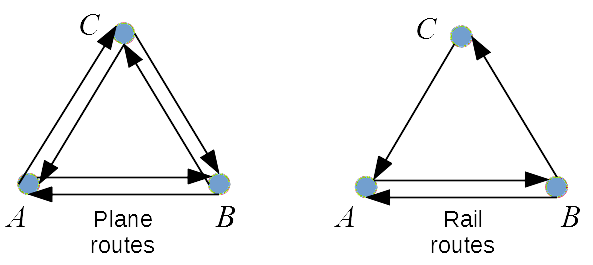
\includegraphics[width=2.5in]{relation-graphs.png}
%{\em Figure 1: Diagrams with Transport Links.}
\end{center}

They have these following truth tables:
\begin{center}
\begin{tabular}{c|ccc}
Plane & $A$ & $B$ & $C$ \\ \hline
$A$ & $\mathtt{F}$ & $\mathtt{T}$ & $\mathtt{T}$ \\
$B$ & $\mathtt{T}$ & $\mathtt{F}$ & $\mathtt{T}$ \\
$C$ & $\mathtt{T}$ & $\mathtt{T}$ & $\mathtt{F}$
\end{tabular}
\hspace{2ex}
\begin{tabular}{c|ccc}
Rail & $A$ & $B$ & $C$ \\ \hline
$A$ & $\mathtt{F}$ & $\mathtt{T}$ & $\mathtt{F}$ \\
$B$ & $\mathtt{T}$ & $\mathtt{F}$ & $\mathtt{T}$ \\
$C$ & $\mathtt{T}$ & $\mathtt{F}$ & $\mathtt{F}$
\end{tabular}
\end{center}
Find the truth values of these statements:\\
{\bf (a)} $\forall x \exists y, \neg P(x,y)$\\
{\bf (b)} $\forall x \forall y \exists z, P(x,z) \wedge P(z,y)$\\
{\bf (c)} $\exists x \exists y \exists z, Q(x,y) \wedge Q(y,z) \wedge Q(z,x)$\\
{\bf (d)} $\forall x \forall y \exists z, Q(x,z) \wedge Q(z,y)$\\
{\em Note.} In the truth tables the first argument is
represented by row, the second is represented by column. 
For example, $\mathrm{Rail}(\mathtt{C}, \mathtt{B}) = \mathtt{F}$ (3rd row,
2nd column).



\vspace{40pt}
{\bf Question 7.} 
Two positive real numbers $x,y \in \mathbb{R}^{+}$ are given. 
Translate into predicate logic this statement:
``Values $x$ and $y$ are the same, if we round them to two 
decimal places.'' In Python this predicate can be written like this:
\begin{verbatim}
def P(x,y):
    return(round(x,ndigits=2) == 
      round(y,ndigits=2))
\end{verbatim}
{\em Note.} Rounding $x$ to two decimal places finds the 
number $\frac{p}{100}$ closest to $x$. 
If two are equally close, then round up.
(For example, $3.14159$ rounds to $3.14$; $3.144999$ rounds to $3.14$, 
but $3.145$ rounds to $3.15$.)




\end{document}



%%%%%%%%%%%%%%%%%%%%%%%%%%%%%%%%%%%%%%%%
%% End of RBS stuff
%%%%%%%%%%%%%%%%%%%%%%%%%%%%%%%%%%%%%%%%


%% 
%% Copyright (C) 2011-2017 by Brian D. Beitzel <brian at beitzel.com>
%% 
%% This work may be distributed and/or modified under the
%% conditions of the LaTeX Project Public License (LPPL), either
%% version 1.3c of this license or (at your option) any later
%% version.  The latest version of this license is in the file:
%% 
%% http://www.latex-project.org/lppl.txt
%% 
%% Users may freely modify these files without permission, as long as the
%% copyright line and this statement are maintained intact.
%% 
%% This work is not endorsed by, affiliated with, or probably even known
%% by, the American Psychological Association.
%% 
%% 
%% This work is "maintained" (as per LPPL maintenance status) by
%% Brian D. Beitzel.
%% 
%% This work consists of the file  apa6.dtx
%% and the derived files           apa6.ins,
%%                                 apa6.cls,
%%                                 apa6.pdf,
%%                                 README,
%%                                 APAamerican.txt,
%%                                 APAbritish.txt,
%%                                 APAdutch.txt,
%%                                 APAenglish.txt,
%%                                 APAgerman.txt,
%%                                 APAngerman.txt,
%%                                 APAgreek.txt,
%%                                 APAczech.txt,
%%                                 APAturkish.txt,
%%                                 APAendfloat.cfg,
%%                                 apa6.ptex,
%%                                 TeX2WordForapa6.bas,
%%                                 Figure1.pdf,
%%                                 shortsample.tex,
%%                                 longsample.tex, and
%%                                 bibliography.bib.
%% 
%%
%% End of file `./samples/shortsample.tex'.
